% Options for packages loaded elsewhere
% Options for packages loaded elsewhere
\PassOptionsToPackage{unicode}{hyperref}
\PassOptionsToPackage{hyphens}{url}
\PassOptionsToPackage{dvipsnames,svgnames,x11names}{xcolor}
%
\documentclass[
  letterpaper,
  DIV=11,
  numbers=noendperiod]{scrartcl}
\usepackage{xcolor}
\usepackage{amsmath,amssymb}
\setcounter{secnumdepth}{-\maxdimen} % remove section numbering
\usepackage{iftex}
\ifPDFTeX
  \usepackage[T1]{fontenc}
  \usepackage[utf8]{inputenc}
  \usepackage{textcomp} % provide euro and other symbols
\else % if luatex or xetex
  \usepackage{unicode-math} % this also loads fontspec
  \defaultfontfeatures{Scale=MatchLowercase}
  \defaultfontfeatures[\rmfamily]{Ligatures=TeX,Scale=1}
\fi
\usepackage{lmodern}
\ifPDFTeX\else
  % xetex/luatex font selection
\fi
% Use upquote if available, for straight quotes in verbatim environments
\IfFileExists{upquote.sty}{\usepackage{upquote}}{}
\IfFileExists{microtype.sty}{% use microtype if available
  \usepackage[]{microtype}
  \UseMicrotypeSet[protrusion]{basicmath} % disable protrusion for tt fonts
}{}
\makeatletter
\@ifundefined{KOMAClassName}{% if non-KOMA class
  \IfFileExists{parskip.sty}{%
    \usepackage{parskip}
  }{% else
    \setlength{\parindent}{0pt}
    \setlength{\parskip}{6pt plus 2pt minus 1pt}}
}{% if KOMA class
  \KOMAoptions{parskip=half}}
\makeatother
% Make \paragraph and \subparagraph free-standing
\makeatletter
\ifx\paragraph\undefined\else
  \let\oldparagraph\paragraph
  \renewcommand{\paragraph}{
    \@ifstar
      \xxxParagraphStar
      \xxxParagraphNoStar
  }
  \newcommand{\xxxParagraphStar}[1]{\oldparagraph*{#1}\mbox{}}
  \newcommand{\xxxParagraphNoStar}[1]{\oldparagraph{#1}\mbox{}}
\fi
\ifx\subparagraph\undefined\else
  \let\oldsubparagraph\subparagraph
  \renewcommand{\subparagraph}{
    \@ifstar
      \xxxSubParagraphStar
      \xxxSubParagraphNoStar
  }
  \newcommand{\xxxSubParagraphStar}[1]{\oldsubparagraph*{#1}\mbox{}}
  \newcommand{\xxxSubParagraphNoStar}[1]{\oldsubparagraph{#1}\mbox{}}
\fi
\makeatother

\usepackage{color}
\usepackage{fancyvrb}
\newcommand{\VerbBar}{|}
\newcommand{\VERB}{\Verb[commandchars=\\\{\}]}
\DefineVerbatimEnvironment{Highlighting}{Verbatim}{commandchars=\\\{\}}
% Add ',fontsize=\small' for more characters per line
\usepackage{framed}
\definecolor{shadecolor}{RGB}{241,243,245}
\newenvironment{Shaded}{\begin{snugshade}}{\end{snugshade}}
\newcommand{\AlertTok}[1]{\textcolor[rgb]{0.68,0.00,0.00}{#1}}
\newcommand{\AnnotationTok}[1]{\textcolor[rgb]{0.37,0.37,0.37}{#1}}
\newcommand{\AttributeTok}[1]{\textcolor[rgb]{0.40,0.45,0.13}{#1}}
\newcommand{\BaseNTok}[1]{\textcolor[rgb]{0.68,0.00,0.00}{#1}}
\newcommand{\BuiltInTok}[1]{\textcolor[rgb]{0.00,0.23,0.31}{#1}}
\newcommand{\CharTok}[1]{\textcolor[rgb]{0.13,0.47,0.30}{#1}}
\newcommand{\CommentTok}[1]{\textcolor[rgb]{0.37,0.37,0.37}{#1}}
\newcommand{\CommentVarTok}[1]{\textcolor[rgb]{0.37,0.37,0.37}{\textit{#1}}}
\newcommand{\ConstantTok}[1]{\textcolor[rgb]{0.56,0.35,0.01}{#1}}
\newcommand{\ControlFlowTok}[1]{\textcolor[rgb]{0.00,0.23,0.31}{\textbf{#1}}}
\newcommand{\DataTypeTok}[1]{\textcolor[rgb]{0.68,0.00,0.00}{#1}}
\newcommand{\DecValTok}[1]{\textcolor[rgb]{0.68,0.00,0.00}{#1}}
\newcommand{\DocumentationTok}[1]{\textcolor[rgb]{0.37,0.37,0.37}{\textit{#1}}}
\newcommand{\ErrorTok}[1]{\textcolor[rgb]{0.68,0.00,0.00}{#1}}
\newcommand{\ExtensionTok}[1]{\textcolor[rgb]{0.00,0.23,0.31}{#1}}
\newcommand{\FloatTok}[1]{\textcolor[rgb]{0.68,0.00,0.00}{#1}}
\newcommand{\FunctionTok}[1]{\textcolor[rgb]{0.28,0.35,0.67}{#1}}
\newcommand{\ImportTok}[1]{\textcolor[rgb]{0.00,0.46,0.62}{#1}}
\newcommand{\InformationTok}[1]{\textcolor[rgb]{0.37,0.37,0.37}{#1}}
\newcommand{\KeywordTok}[1]{\textcolor[rgb]{0.00,0.23,0.31}{\textbf{#1}}}
\newcommand{\NormalTok}[1]{\textcolor[rgb]{0.00,0.23,0.31}{#1}}
\newcommand{\OperatorTok}[1]{\textcolor[rgb]{0.37,0.37,0.37}{#1}}
\newcommand{\OtherTok}[1]{\textcolor[rgb]{0.00,0.23,0.31}{#1}}
\newcommand{\PreprocessorTok}[1]{\textcolor[rgb]{0.68,0.00,0.00}{#1}}
\newcommand{\RegionMarkerTok}[1]{\textcolor[rgb]{0.00,0.23,0.31}{#1}}
\newcommand{\SpecialCharTok}[1]{\textcolor[rgb]{0.37,0.37,0.37}{#1}}
\newcommand{\SpecialStringTok}[1]{\textcolor[rgb]{0.13,0.47,0.30}{#1}}
\newcommand{\StringTok}[1]{\textcolor[rgb]{0.13,0.47,0.30}{#1}}
\newcommand{\VariableTok}[1]{\textcolor[rgb]{0.07,0.07,0.07}{#1}}
\newcommand{\VerbatimStringTok}[1]{\textcolor[rgb]{0.13,0.47,0.30}{#1}}
\newcommand{\WarningTok}[1]{\textcolor[rgb]{0.37,0.37,0.37}{\textit{#1}}}

\usepackage{longtable,booktabs,array}
\newcounter{none} % for unnumbered tables
\usepackage{calc} % for calculating minipage widths
% Correct order of tables after \paragraph or \subparagraph
\usepackage{etoolbox}
\makeatletter
\patchcmd\longtable{\par}{\if@noskipsec\mbox{}\fi\par}{}{}
\makeatother
% Allow footnotes in longtable head/foot
\IfFileExists{footnotehyper.sty}{\usepackage{footnotehyper}}{\usepackage{footnote}}
\makesavenoteenv{longtable}
\usepackage{graphicx}
\makeatletter
\newsavebox\pandoc@box
\newcommand*\pandocbounded[1]{% scales image to fit in text height/width
  \sbox\pandoc@box{#1}%
  \Gscale@div\@tempa{\textheight}{\dimexpr\ht\pandoc@box+\dp\pandoc@box\relax}%
  \Gscale@div\@tempb{\linewidth}{\wd\pandoc@box}%
  \ifdim\@tempb\p@<\@tempa\p@\let\@tempa\@tempb\fi% select the smaller of both
  \ifdim\@tempa\p@<\p@\scalebox{\@tempa}{\usebox\pandoc@box}%
  \else\usebox{\pandoc@box}%
  \fi%
}
% Set default figure placement to htbp
\def\fps@figure{htbp}
\makeatother





\setlength{\emergencystretch}{3em} % prevent overfull lines

\providecommand{\tightlist}{%
  \setlength{\itemsep}{0pt}\setlength{\parskip}{0pt}}



 


\KOMAoption{captions}{tableheading}
\makeatletter
\@ifpackageloaded{caption}{}{\usepackage{caption}}
\AtBeginDocument{%
\ifdefined\contentsname
  \renewcommand*\contentsname{Table of contents}
\else
  \newcommand\contentsname{Table of contents}
\fi
\ifdefined\listfigurename
  \renewcommand*\listfigurename{List of Figures}
\else
  \newcommand\listfigurename{List of Figures}
\fi
\ifdefined\listtablename
  \renewcommand*\listtablename{List of Tables}
\else
  \newcommand\listtablename{List of Tables}
\fi
\ifdefined\figurename
  \renewcommand*\figurename{Figure}
\else
  \newcommand\figurename{Figure}
\fi
\ifdefined\tablename
  \renewcommand*\tablename{Table}
\else
  \newcommand\tablename{Table}
\fi
}
\@ifpackageloaded{float}{}{\usepackage{float}}
\floatstyle{ruled}
\@ifundefined{c@chapter}{\newfloat{codelisting}{h}{lop}}{\newfloat{codelisting}{h}{lop}[chapter]}
\floatname{codelisting}{Listing}
\newcommand*\listoflistings{\listof{codelisting}{List of Listings}}
\makeatother
\makeatletter
\makeatother
\makeatletter
\@ifpackageloaded{caption}{}{\usepackage{caption}}
\@ifpackageloaded{subcaption}{}{\usepackage{subcaption}}
\makeatother
\usepackage{bookmark}
\IfFileExists{xurl.sty}{\usepackage{xurl}}{} % add URL line breaks if available
\urlstyle{same}
\hypersetup{
  pdftitle={OEKA201AssignmentOPAMPJ},
  pdfauthor={Andreas Moen; Oskar Petterson; Philip Jacobsen},
  pdfkeywords={Wine Prices, Regression Analysis, R Programming, Quarto,
Data Analysis},
  colorlinks=true,
  linkcolor={blue},
  filecolor={Maroon},
  citecolor={Blue},
  urlcolor={Blue},
  pdfcreator={LaTeX via pandoc}}


\title{OEKA201AssignmentOPAMPJ}
\author{Andreas Moen \and Oskar Petterson \and Philip Jacobsen}
\date{}
\begin{document}
\maketitle
\begin{abstract}
This mini-thesis analyzes \ldots.
\end{abstract}

\renewcommand*\contentsname{Table of contents}
{
\setcounter{tocdepth}{3}
\tableofcontents
}
\listoffigures
\listoftables

\begin{Shaded}
\begin{Highlighting}[]
\FunctionTok{source}\NormalTok{(}\StringTok{"script/estm.R"}\NormalTok{)}
\end{Highlighting}
\end{Shaded}

\begin{verbatim}

Call:
lm(formula = salary ~ education_level, data = df)

Residuals:
    Min      1Q  Median      3Q     Max 
-113153  -24825   -1921   22695  169070 

Coefficients:
                           Estimate Std. Error t value Pr(>|t|)    
(Intercept)                142410.5      159.2  894.79   <2e-16 ***
education_levelDiploma      -5252.0      225.3  -23.31   <2e-16 ***
education_levelHigh School -10695.2      225.0  -47.55   <2e-16 ***
education_levelMaster       10894.8      224.6   48.50   <2e-16 ***
education_levelPhD          21565.5      225.2   95.77   <2e-16 ***
---
Signif. codes:  0 '***' 0.001 '**' 0.01 '*' 0.05 '.' 0.1 ' ' 1

Residual standard error: 35570 on 249995 degrees of freedom
Multiple R-squared:  0.09584,   Adjusted R-squared:  0.09583 
F-statistic:  6625 on 4 and 249995 DF,  p-value: < 2.2e-16


Call:
lm(formula = salary ~ education_level + experience_years + industry, 
    data = df)

Residuals:
    Min      1Q  Median      3Q     Max 
-107845  -20898   -1398   20007  144375 

Coefficients:
                            Estimate Std. Error t value Pr(>|t|)    
(Intercept)                115193.60     257.35 447.608   <2e-16 ***
education_levelDiploma      -5253.98     199.95 -26.277   <2e-16 ***
education_levelHigh School -10658.11     199.66 -53.382   <2e-16 ***
education_levelMaster       11014.40     199.38  55.244   <2e-16 ***
education_levelPhD          21614.77     199.87 108.145   <2e-16 ***
experience_years             2703.96      10.42 259.533   <2e-16 ***
industryEducation             331.60     281.98   1.176    0.240    
industryFinance               221.56     280.57   0.790    0.430    
industryGovernment            205.41     281.94   0.729    0.466    
industryHealthcare            167.25     281.95   0.593    0.553    
industryManufacturing        -125.84     281.59  -0.447    0.655    
industryMedia                 345.84     281.56   1.228    0.219    
industryRetail               -371.28     282.11  -1.316    0.188    
industryTechnology            182.57     281.94   0.648    0.517    
industryTelecom               259.47     282.06   0.920    0.358    
---
Signif. codes:  0 '***' 0.001 '**' 0.01 '*' 0.05 '.' 0.1 ' ' 1

Residual standard error: 31570 on 249985 degrees of freedom
Multiple R-squared:  0.2878,    Adjusted R-squared:  0.2877 
F-statistic:  7215 on 14 and 249985 DF,  p-value: < 2.2e-16


Call:
lm(formula = salary ~ education_level + experience_years + remote_work, 
    data = df)

Residuals:
    Min      1Q  Median      3Q     Max 
-106068  -20830   -1418   19937  145964 

Coefficients:
                            Estimate Std. Error t value Pr(>|t|)    
(Intercept)                113482.92     196.57  577.32   <2e-16 ***
education_levelDiploma      -5271.56     199.32  -26.45   <2e-16 ***
education_levelHigh School -10658.30     199.03  -53.55   <2e-16 ***
education_levelMaster       10990.52     198.75   55.30   <2e-16 ***
education_levelPhD          21603.40     199.24  108.43   <2e-16 ***
experience_years             2704.41      10.39  260.40   <2e-16 ***
remote_workNo                 141.66     153.98    0.92    0.358    
remote_workYes               5401.37     154.31   35.00   <2e-16 ***
---
Signif. codes:  0 '***' 0.001 '**' 0.01 '*' 0.05 '.' 0.1 ' ' 1

Residual standard error: 31470 on 249992 degrees of freedom
Multiple R-squared:  0.2922,    Adjusted R-squared:  0.2922 
F-statistic: 1.475e+04 on 7 and 249992 DF,  p-value: < 2.2e-16
\end{verbatim}

\section{Topic of interest: The correlation between salary and higher
education.}\label{topic-of-interest-the-correlation-between-salary-and-higher-education.}

Research question: Does higher education lead to higer salary?

Our research question: Does higher education lead to higher salary? Is
central to labor economics and has been explored a lot in academic
literature over the years.~~

A big contribution to this field is Blaug (1972), who examines the
correlation between education and earnings in his article The
correlation between education and earnings:~

What does it signify? Referance:
\url{https://link.springer.com/article/10.1007/BF01956881}

Dataset:
\url{https://www.kaggle.com/datasets/nalisha/job-salary-prediction-dataset}~

\href{https://link.springer.com/article/10.1007/BF01956881}{The
correlation between education and earnings: What does it signify? -
Higher Education}~

\href{https://link.springer.com/article/10.1007/BF01956881}{link.springer.com}~

The dataset used in this analysis is stored in the package folder under
data-raw/job\_salary\_prediction\_dataset.csv. The dataset contains
250,000 observations and 10 variables, including education level,
experience, job title, industry, company size, and salary.

1. Data Description \& Summary~Open your selected data set in Gretl and
provide a brief summary using descriptive statistics and graphical
representations of key variables. Relate the analysis to your RQ.

\pandocbounded{\includegraphics[keepaspectratio]{assignment_r_files/mediabag/9we7fAAAAABklEQVQDAA.png}}

\section{2. Simple Regression Model: Estimate a simple regression model
where you define your dependent and indepen-dent variable based on your
RQ.~}\label{simple-regression-model-estimate-a-simple-regression-model-where-you-define-your-dependent-and-indepen-dent-variable-based-on-your-rq.}

a) Present the output from your analysis.

From the output we have 250 000 observations and~ the dependent variable
is the salary. The key results from the regression model is given
as.:~\\

{\def\LTcaptype{none} % do not increment counter
\begin{longtable}[]{@{}
  >{\raggedright\arraybackslash}p{(\linewidth - 8\tabcolsep) * \real{0.2500}}
  >{\raggedright\arraybackslash}p{(\linewidth - 8\tabcolsep) * \real{0.1944}}
  >{\raggedright\arraybackslash}p{(\linewidth - 8\tabcolsep) * \real{0.1806}}
  >{\raggedright\arraybackslash}p{(\linewidth - 8\tabcolsep) * \real{0.1389}}
  >{\raggedright\arraybackslash}p{(\linewidth - 8\tabcolsep) * \real{0.2361}}@{}}
\toprule\noalign{}
\endhead
\bottomrule\noalign{}
\endlastfoot
Variable~ & Coefficient~ & Std. Error~ & t-value~ & p-value~ \\
Constant~ & 147 168~ & 175.45~ & 838.8~ & 0.000~ \\
Education Level~ & -482.9~ & 52.85~ & -9.14~ & 6.45*10\^{}-20~~ \\
\end{longtable}
}

We also have a R squared value of 0.000334 and a F statistic p value of
\[6.45*10^-20\] ~

We can see there is a big significance between salary and education
level.

b) Interpret the estimated coefficients.~

The constant is estimated as 147168. This represents the yearly
predicted salary to a person at the lowest educational level in the
dataset. The coefficient for the education level is estimated to
--482,9. This shows that for every additional step in the education the
salary is expected to be 482.9 lower.~

c) Evaluate the significance of the independent variable(s) at a 5\%
significance~

level.~~

We can clearly see that \[6.45*10^-20 is < 0.05\] so the variable is
statistically very significant. Even though its significant the R
squared value is very low, which can be interpretated as the model not
explaining the variation in the salary.~~

d) Make predictions using the model at different values of an
independent variable.~

We just plug in different variables for the education level. After we
ran the simple regression model we got this equation:
\[salary = 147168 + (-482,90) × education_level\]. By using this
equation we can predict the salary based on the education levels.

{\def\LTcaptype{none} % do not increment counter
\begin{longtable}[]{@{}ll@{}}
\toprule\noalign{}
\endhead
\bottomrule\noalign{}
\endlastfoot
Education\_level~ & Predicted salary~ \\
1~ & 146 685~ \\
2~ & 146 202~ \\
3~ & 145 719~ \\
4~ & 145 236~ \\
5~ & 144 753~ \\
\end{longtable}
}

This table shows that the predicted salary is getting lower by every
education level. The results in the simple regression shows that there
are negative correlation between salary and education level, to
contradict our research question of whether higher education leads to
higher salary. The model only includes education as an explanatory
variable and does not control for other important factors such as work
experience, skills and industry.~

e) Calculate a 95\% prediction interval for a specific observation in
your context.~

A 95\% prediciton interval for a specific observation can be calculated
as the predicted values plus or minus a critical value times the
prediction standard error. Using the regression output the standard
error of regression is 37401.78. So when education levels equals to 5
the predicted salery is.:~

\[
Salery=147168-482.9(5)
\]

\[
salery=147168-2414.5=144753.5
\]

Then the approximate 95\% prediciton interval:

\[
1.96*37401.78=73307,49
\]

so that gives us

So lower bound = 71 446.01

And upper bound = 218060.99 so the approximate 95\% prediction interval
is given as.:

(71446.01, 218060.99)

This means that the actual salary for an individual with education level
5 is expected to lie within thhis interval with 95\% confidence.

\section{3. Multiple Regression Model}\label{multiple-regression-model}

\section{Script Showcasing}\label{script-showcasing}

You can find the script in the script folder.

\begin{Shaded}
\begin{Highlighting}[]
\InformationTok{\textasciigrave{}\textasciigrave{}\textasciigrave{}\{r\}}
\FunctionTok{library}\NormalTok{(OEKA201AssignmentOPAMPJ)}
\CommentTok{\# Load dataset}
\NormalTok{df}\CommentTok{\# \textless{}{-} read.csv("data{-}raw/job\_salary\_prediction\_dataset.csv")}

\CommentTok{\# Convert categorical variables to factors}
\NormalTok{df}\SpecialCharTok{$}\NormalTok{education\_level }\OtherTok{\textless{}{-}} \FunctionTok{as.factor}\NormalTok{(df}\SpecialCharTok{$}\NormalTok{education\_level)}
\NormalTok{df}\SpecialCharTok{$}\NormalTok{industry }\OtherTok{\textless{}{-}} \FunctionTok{as.factor}\NormalTok{(df}\SpecialCharTok{$}\NormalTok{industry)}
\NormalTok{df}\SpecialCharTok{$}\NormalTok{remote\_work }\OtherTok{\textless{}{-}} \FunctionTok{as.factor}\NormalTok{(df}\SpecialCharTok{$}\NormalTok{remote\_work)}

\CommentTok{\# 1. Simple regression}
\NormalTok{model\_simple }\OtherTok{\textless{}{-}} \FunctionTok{lm}\NormalTok{(salary }\SpecialCharTok{\textasciitilde{}}\NormalTok{ education\_level, }\AttributeTok{data =}\NormalTok{ df)}

\CommentTok{\# 2. Multiple regression}
\NormalTok{model\_multiple }\OtherTok{\textless{}{-}} \FunctionTok{lm}\NormalTok{(salary }\SpecialCharTok{\textasciitilde{}}\NormalTok{ education\_level }\SpecialCharTok{+}\NormalTok{ experience\_years }\SpecialCharTok{+}\NormalTok{ industry, }\AttributeTok{data =}\NormalTok{ df)}

\CommentTok{\# 3. Dummy variable model with remote work}
\NormalTok{model\_dummy }\OtherTok{\textless{}{-}} \FunctionTok{lm}\NormalTok{(salary }\SpecialCharTok{\textasciitilde{}}\NormalTok{ education\_level }\SpecialCharTok{+}\NormalTok{ experience\_years }\SpecialCharTok{+}\NormalTok{ remote\_work, }\AttributeTok{data =}\NormalTok{ df)}

\CommentTok{\# Show results}
\FunctionTok{print}\NormalTok{(}\FunctionTok{summary}\NormalTok{(model\_simple))}
\FunctionTok{print}\NormalTok{(}\FunctionTok{summary}\NormalTok{(model\_multiple))}
\FunctionTok{print}\NormalTok{(}\FunctionTok{summary}\NormalTok{(model\_dummy))}



\InformationTok{\textasciigrave{}\textasciigrave{}\textasciigrave{}}
\end{Highlighting}
\end{Shaded}

Expand your model by including additional relevant variables.

a) Explain the choice of additional variables

We wanted to see how the industry, education level and experience have a
correlation with salary. And it seems that there is a significant
between education level, experience but not a big correlation with
industry. Which make sense as you can have high and low salaries in all
kinds of industry fields.

b) Present the output from your
analysis.\pandocbounded{\includegraphics[keepaspectratio]{assignment_r_files/mediabag/NRZgb52Nz4ODdP3cWmKM.png}}

c) Interpret the estimated slope coefficients.

Based on the results from our new regression model, Education level:
-463,991.

When we keep the experience years and the industry constant, the
predicted salary drops by 464 units from every additional education
level. This indicates a negative correlation between education and
salary in this data set.

Experience years: 2700,99. When we keep the education level and the
indusrty constant the expected yearly salary rises with 2701 units. This
indicates an extremely positve effect on the yearly salary which makes
sense.

Industry: -14-5. The P value is too high to really consider this and we
can't really use this data, because it is very random and we dont have
enough proof.

d) Evaluate the significance of the independent variable(s) at a 5\%
significance Level.

Like mentioned previously the education level, and experience in years
have a very strong statistically significant as p value \textless{}
0.05. However the industry have a p value of 0.536 \textgreater{} 0.05
so it's not statistically significant.

At the 5\% significance level, the variables education level and
experience years are statistically significant, as their p values are
far below 0.05 (close to 0.00). Which means both variables have a
significant effect on salary. In contrast the variable industry has a p
value of 0.536 which is greater than 0.05 indicating that its not
statistically significant. Therefore, there is no evidence that industry
affects salary in this model.

e) Compare the results to your simple regression analysis.

Compared to the simple regression model the multipåle regression model
provides a much better fit to the data. The R Squared increases
significantly from 0.000334 to 0.1918 indicating that the model explains
a muchg larger share of the variation in salary. The coefficient for
education level remains negative and statistically significant, but its
magnitude decreases slightly when additional variables are included.
This suggests that the simple model may suffer from omitted variable
bias, particularly due to the exclusion of experience. Furthermore,
experience years is highly significant and has a strong positive effect
on salary, while the industry variable is not statistically significant.
Overall, the multiple regression model is more reliable and provides a
better explanation of salary differences.

\section{4-1. Dummy Variable Analysis}\label{dummy-variable-analysis}

Identify a situation where a dummy variable could be used in your data
(e.g., an

event or using thresholds to generate groups). Create (if needed) and
use this dummy

variable in a regression model. Use it to estimate a fixed effect, an
interaction effect,

or a combination of both - whichever is more suitable for your project.

\pandocbounded{
\includegraphics[keepaspectratio]{images/clipboard-1944769457.png}}

a) Present the output from your analysis.

Dummy variables are used to represent categorical variables in the
regression model. In this case, remote work is divided into three
categories.: Hybrid, NO and YES. Hybrid is only used as the reference
category, while two dummy variables are included.: One for remote work =
YES and one for remote work = NO

The constant term represents the average salary for individuals working
in a hybrid arrangement. The coefficient for remote work = YES is
5309.69 and is statistically significant, indicating that fully remote
workers earn on average about 5309 more than hybrid workers. The
coefficient for remote work = NO is not statistically significant
suggesting no meaningful difference in salary compared to hybrid
workers.

b) Discuss the impact of this dummy variable on your dependent variable,
considering any interaction effects.

The dummy variables for remote work capture differences in salary
relative to the reference category, which is hybrid work. The Results
show that individuals who work fully remotely earn on average about 5309
of X currency more than hybrid workers, and this effect is statistically
significant. In contract, individuals who do not work remotely have a
small and statistically insignificant difference in salary compared to
hybrid workers indicating no meaningful effect.

These results suggest that remote work may be associated with higher
paying jobs, while there is no clear difference between hybrid and fully
on-site work. The model does not include any interaction terms, meaning
that the effect of remote work is assumed to be constant across all
indivduals. The impact of remote work may vary dpeneing on factors such
as experience or education, but this is not captured in the current
specification.

\section{5. Model Selection and
Analysis}\label{model-selection-and-analysis}

a) Use the different models to predict the dependent variable in for a
given state

of the independent variables

\pandocbounded{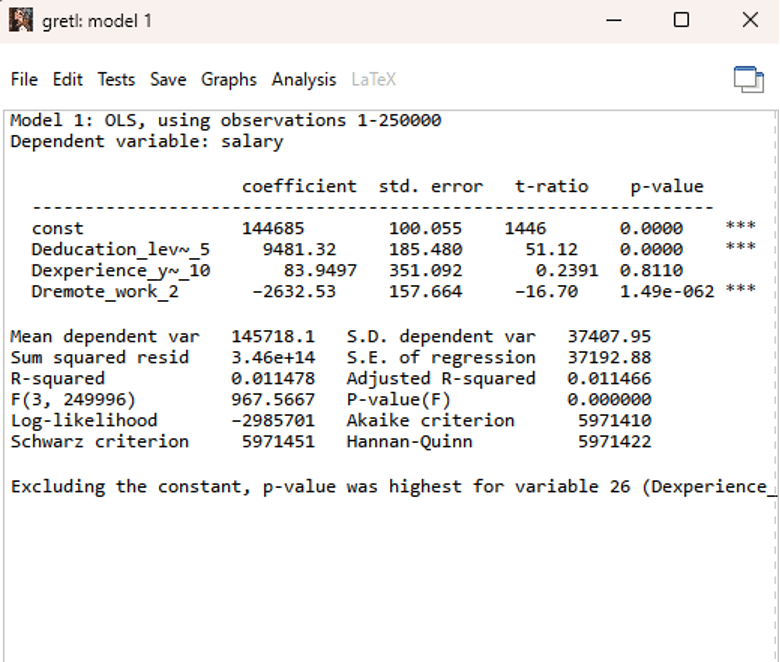
\includegraphics[keepaspectratio]{images/clipboard-1128260562.png}}

Model number 1 has master degree, 10 years of work experience and works
on site.

We can see that the master degree has the biggest impact on his/her
salary. With a significance value of 0.000. Compared to the others, we
can see that 10 years of experience is not significant with a p value of
0.8110 and working on site has a negative effect on the salary with a
very high signifance p value of 0.00\ldots1.49

This person will have a salary of
\[ 144 685 + 9 481 + 83,95 - 2 633 = 151 617\]

This means the expected salary is approximately 151 618 in X currency.
The master degree has a strong positive and statistically significant
effect on salary, increasing it by about 9481, compared to the reference
group. The effect of having 10 years of experience is small and not
statistically significant, indicating no meaningful impact. Working on
site is associated with a decrease in salary of about 2633 compared to
the reference category and is statistically significant.

\pandocbounded{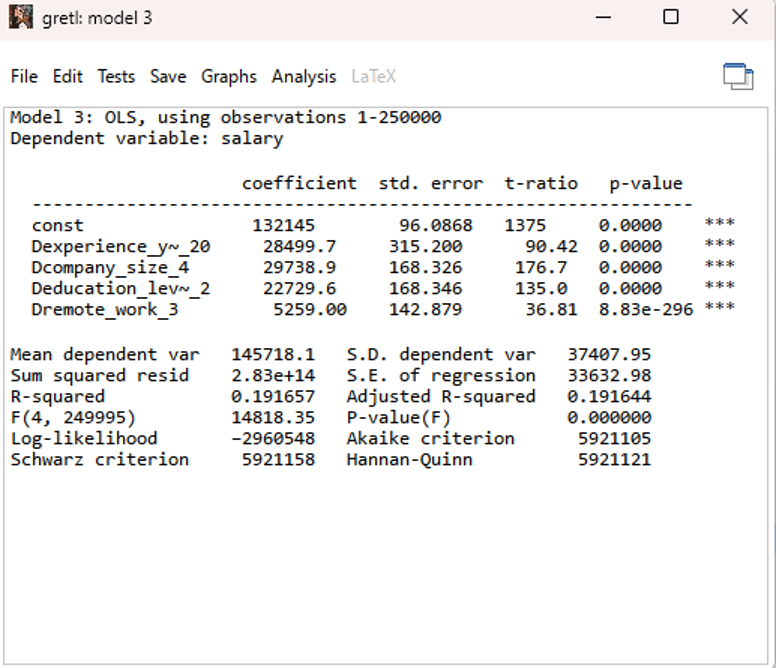
\includegraphics[keepaspectratio]{images/clipboard-640619700.png}}

For model number 2 we have 20 years of experience, a PHD degree and
he/her is working in an enterprise and working from home.

THis corresponds to an expected salary of approximately 218 372. All
included variables have a positive and statistically significant effects
on salary. In particular working from home increases the salary by about
5259 compared to the reference category holding others factors constant.
The R squared value tells us that 19.17\% of the variation in salary is
explained by the model. More of the model can be explained if we add
what country and what type of field the person is working in.

b) Based on these analyses and additional considerations (e.g., model
fit, theoretical soundness), discuss which model you would prefer for
predicting outcomes within your context and why.

\section{Conclusion}\label{conclusion}

We prefer model 2 because it has the highest R² which is 19,2\%,
compared to the other models that is far lower than this. A higher R²
explains a bigger portion of the variation in the salary making it more
accurate and gives us the most accurate information. The model does not
explain all variation, but it gives us a reliable estimate and most
accurate comparing to the other models we have used.

\section{Appendix}\label{appendix}

\begin{Shaded}
\begin{Highlighting}[]
\InformationTok{\textasciigrave{}\textasciigrave{}\textasciigrave{}\{r\}}
\FunctionTok{library}\NormalTok{(OEKA201AssignmentOPAMPJ)}
\CommentTok{\# Load dataset}
\NormalTok{df}\CommentTok{\# \textless{}{-} read.csv("data{-}raw/job\_salary\_prediction\_dataset.csv")}

\CommentTok{\# Convert categorical variables to factors}
\NormalTok{df}\SpecialCharTok{$}\NormalTok{education\_level }\OtherTok{\textless{}{-}} \FunctionTok{as.factor}\NormalTok{(df}\SpecialCharTok{$}\NormalTok{education\_level)}
\NormalTok{df}\SpecialCharTok{$}\NormalTok{industry }\OtherTok{\textless{}{-}} \FunctionTok{as.factor}\NormalTok{(df}\SpecialCharTok{$}\NormalTok{industry)}
\NormalTok{df}\SpecialCharTok{$}\NormalTok{remote\_work }\OtherTok{\textless{}{-}} \FunctionTok{as.factor}\NormalTok{(df}\SpecialCharTok{$}\NormalTok{remote\_work)}

\CommentTok{\# 1. Simple regression}
\NormalTok{model\_simple }\OtherTok{\textless{}{-}} \FunctionTok{lm}\NormalTok{(salary }\SpecialCharTok{\textasciitilde{}}\NormalTok{ education\_level, }\AttributeTok{data =}\NormalTok{ df)}

\CommentTok{\# 2. Multiple regression}
\NormalTok{model\_multiple }\OtherTok{\textless{}{-}} \FunctionTok{lm}\NormalTok{(salary }\SpecialCharTok{\textasciitilde{}}\NormalTok{ education\_level }\SpecialCharTok{+}\NormalTok{ experience\_years }\SpecialCharTok{+}\NormalTok{ industry, }\AttributeTok{data =}\NormalTok{ df)}

\CommentTok{\# 3. Dummy variable model with remote work}
\NormalTok{model\_dummy }\OtherTok{\textless{}{-}} \FunctionTok{lm}\NormalTok{(salary }\SpecialCharTok{\textasciitilde{}}\NormalTok{ education\_level }\SpecialCharTok{+}\NormalTok{ experience\_years }\SpecialCharTok{+}\NormalTok{ remote\_work, }\AttributeTok{data =}\NormalTok{ df)}

\CommentTok{\# Show results}
\FunctionTok{print}\NormalTok{(}\FunctionTok{summary}\NormalTok{(model\_simple))}
\FunctionTok{print}\NormalTok{(}\FunctionTok{summary}\NormalTok{(model\_multiple))}
\FunctionTok{print}\NormalTok{(}\FunctionTok{summary}\NormalTok{(model\_dummy))}



\InformationTok{\textasciigrave{}\textasciigrave{}\textasciigrave{}}
\end{Highlighting}
\end{Shaded}





\end{document}
